\section{Wyznaczanie macierzy sztywności i mas elementów}
\label{sec:wyznaczanie_macierzy}

Weźmy model jednorodnego pręta, obciążonego jak na rysunku \ref{fig:pret} o module Younga \( E \), polu przekroju \( A \) i długości \( L \).

\begin{figure}[h]
\centering
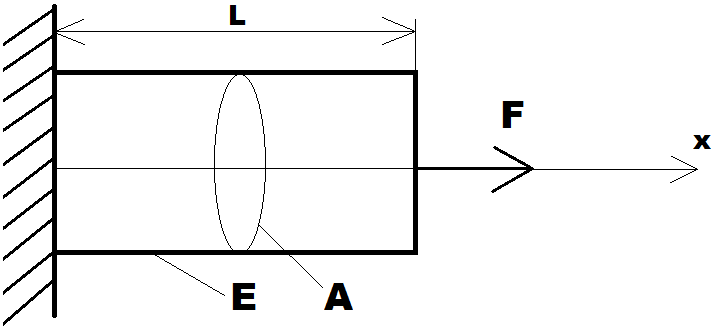
\includegraphics[width=10cm]{Zdjecia/3/pret}
\caption{Model pręta}
\label{fig:pret}
\end{figure}

Energię potencjalną i kinetyczną układu można wyrazić poniższymi wzorami.

\begin{gather} \label{eq:energia}
V = \frac{1}{2} \int_0^L \varepsilon A \sigma dx - Fu_{x=L} = \frac{1}{2} \int_0^L EA {\bigg( \frac{du}{dx}\bigg)}^2 dx - Fu_{x=L} \\
K = \frac{1}{2} \int_0^L \rho A {\bigg(\frac{\partial u}{\partial t}\bigg)}^2 dx
\end{gather}

gdzie
\begin{eqwhere}[2cm]
	\item[$V $] energia potencjalna
	\item[$K $] energia kinetyczna
	\item[$u $] przemieszczenie
	\item[$\varepsilon $] odkształcenie
	\item[$\sigma $] naprężenie
	\item[$F $] siła zewnętrzna skupiona
\end{eqwhere}
	
	Następnie stwórzmy uproszczony model, do którego wyznaczymy zależności MES.

\begin{figure}[h]
\centering
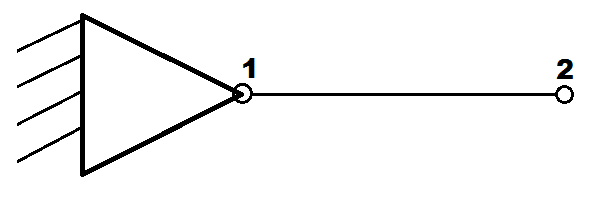
\includegraphics[width=10cm]{Zdjecia/3/pret_upr}
\caption{Uproszczony model pręta}
\label{fig:pret_upr}
\end{figure}

Znając funkcje kształtu i wartości przemieszczeń węzłów można wyznaczyć przemieszczenie w każdym punkcie pręta, a następnie odpowiednie pochodne po przemieszczeniach i po czasie.

\begin{gather}
u = N_1 x_1 + N_2 x_2 = 
	\begin{bmatrix} 
	 	N_1 & N_2 \\
	\end{bmatrix}
	\begin{bmatrix} 
	 	u_1 \\
		u_2 \\
	\end{bmatrix}
\end{gather}

\begin{gather}
\frac{\partial u}{\partial x}= 
	\begin{bmatrix} 
	 	\frac{d N_1}{d x} & \frac{d N_2}{d x} \\
	\end{bmatrix}
	\begin{bmatrix} 
	 	u_1 \\
		u_2 \\
	\end{bmatrix} = \textbf{B u}^e
\end{gather}


\begin{gather}
\frac{\partial u}{\partial t}= 
	\begin{bmatrix} 
	 	N_1 &  N_2 & \\
	\end{bmatrix}
	\begin{bmatrix} 
	 	\frac{du_1}{dt} \\
		\frac{du_2}{dt}\\
	\end{bmatrix} = \textbf{N} \dot{\textbf{u}}^e
\end{gather}


	Mając wyznaczoną energię, możemy obliczyć lagranżjan i wstawić go do dynamicznych równań Lagrangea drugiego rodzaju. Dzięki tej operacji otrzymamy końcowe, dynamiczne równanie ruchu oraz postać macierzy mas i sztywności. Równania Lagrangea drugiego rodzaju mają postać:

\begin{equation}
\frac{d}{dt} \frac{\partial L}{\partial \dot{\textbf{u}}^e} - \frac{\partial L}{\partial \textbf{u}^e} = 0, \quad L = K - V
\end{equation}

gdzie
\begin{eqwhere}[2cm]
	\item[$L$] lagranżjan.
\end{eqwhere}

Pierwszy człon wynosi

\begin{equation}
\frac{d}{dt} \frac{\partial L}{\partial \dot{\textbf{u}}^e} = \int_0^L \rho A {\textbf{N}}^T \textbf{N} {\ddot{\textbf{u}}}^e dx,
\end{equation}

zaś drugi

\begin{equation}
 \frac{\partial L}{\partial \textbf{u}^e} = -\int_0^L EA {\textbf{B}}^T \textbf{B} {\textbf{u}}^e dx + F \textbf{Nu}^e_{x=L}.
\end{equation}

Równanie dynamiki układu zapisane jest poniżej.

\begin{equation}
\int_0^L \rho A {\textbf{N}}^T \textbf{N} dx {\ddot{\textbf{u}}}^e + \int_0^L A {\textbf{B}}^T E \textbf{B} dx u = F \textbf{Nu}^e_{x=L}
\end{equation}

Postaci macierzy mas i sztywności są następujące:

\begin{gather}
\textbf{M}^e = \int_0^L \rho A {\textbf{N}}^T \textbf{N} dx \\
\textbf{K}^e = \int_0^L A {\textbf{B}}^T E \textbf{B} dx.
\end{gather}

W przypadku kiedy występuje więcej niż jedna stała materiałowa, zamiast \( E \) pojawia się macierz materiałowa \( D \). W przypadku bardziej złożonych obiektów o większej liczbie elementów skończonych, całkowanie niezbędne do obliczenia macierzy staje się bardzo czasochłonne. Ponieważ funkcje kształtu są wielomianami, optymalnym rozwiązaniem jest zastosowanie kwadratur Gaussa. Kolejny problem to określenie granic całkowania. W przypadku przedstawionym powyżej nie widać specjalnej trudności, natomiast dla trójwymiarowych obiektów o nieregularnych kształtach wymaga to dodatkowej serii obliczeń.

W takich przypadkach można zastosować mapowanie na współrzędne naturalne. W takich współrzędnych element ma z góry ustalone współrzędne węzłów, co za tym idzie także granice całkowania są znane. Dla obiektu trójwymiarowego przyjmijmy współrzędne rzeczywiste \( x, y, z \) i współrzędne naturalne \( \xi, \eta, \zeta \). Mapowania z jednych współrzędnych na drugie oblicza się według poniższego wzoru. Wizualizacja procedury przedstawiona jest na rysunku \ref{fig:izoparam}.


\begin{gather}
	\begin{bmatrix} 
	 	x \\
		y \\
		z 
	\end{bmatrix} = \sum_{i=1}^n
	\begin{bmatrix} 
	 	x_i \\
		y_i \\
		z_i 
	\end{bmatrix} N_i(\xi, \eta, \zeta)
\end{gather}

\begin{eqwhere}[2cm]
	\item[$x_i, y_i, z_i$] współrzędne rzeczywiste punktów
	\item[$N_i$] funkcje kształtu we współrzędnych naturalnych
	\item[$n$] liczba węzłów elementu.
\end{eqwhere}

\begin{figure}[h]
\centering
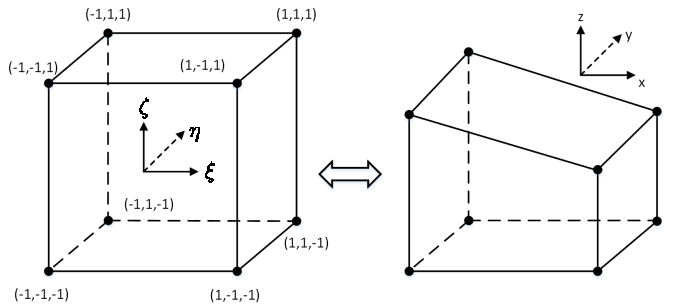
\includegraphics[width=10cm]{Zdjecia/3/izoparam}
\caption{Przekształcenie izoparametryczne}
\label{fig:izoparam}
\end{figure}

Dla elementów w takich współrzędnych funkcje kształtu są znane i stabelaryzowane. Dla elementu sześciennego wypisane są w \ref{eq:f_ksztaltu_hex}.

\begin{equation} \label{eq:f_ksztaltu_hex}
	\begin{aligned}
		N_1 = \frac{1}{8}(1-\xi)(1-\eta)(1-\zeta) \\
		N_2 = \frac{1}{8}(1+\xi)(1-\eta)(1-\zeta) \\
		N_3 = \frac{1}{8}(1+\xi)(1+\eta)(1-\zeta) \\
		N_4 = \frac{1}{8}(1-\xi)(1+\eta)(1-\zeta) \\
		N_5 = \frac{1}{8}(1-\xi)(1-\eta)(1+\zeta) \\
		N_6 = \frac{1}{8}(1+\xi)(1-\eta)(1+\zeta) \\
		N_7 = \frac{1}{8}(1+\xi)(1+\eta)(1+\zeta) \\
		N_8 = \frac{1}{8}(1-\xi)(1+\eta)(1+\zeta)
	\end{aligned}
\end{equation}

Ostatnim elmentem niezbędnym do prawidłowego całkowania we współrzędnych naturalnych jest wyznaczenie jakobianu przekształcenia. Macierz Jacobiego przedstawiona jest w równaniu \ref{eq:m_jacobiego}.

\begin{gather} \label{eq:m_jacobiego}
	\textbf{J} = \begin{bmatrix} 
	 	\frac{\partial x}{\partial \xi} & \frac{\partial y}{\partial \xi} & \frac{\partial z}{\partial \xi} \\
	 	\frac{\partial x}{\partial \eta} & \frac{\partial y}{\partial \eta} & \frac{\partial z}{\partial \eta} \\
	 	\frac{\partial x}{\partial \zeta} & \frac{\partial y}{\partial \zeta} & \frac{\partial z}{\partial \zeta}
	\end{bmatrix}
\end{gather}

Ostatecznie wyznaczanie macierzy mas i sztywności dla elementu sześciennego zostanie zmodyfikowane jak poniżej:

\begin{equation} \label{eq:f_ksztaltu_hex}
	\begin{aligned}
	\textbf{M}^e = \int_V \rho {\textbf{N}}^T \textbf{N} dV \quad \rightarrow \quad \textbf{M}^e = \int_{-1}^1 \int_{-1}^1 \int_{-1}^1 \rho {\textbf{N}}^T \textbf{N} det\textbf{J} d\xi d\eta d\zeta \\
	\textbf{K}^e = \int_V {\textbf{B}}^T E \textbf{B} dV \quad \rightarrow \quad \textbf{K}^e =  \int_{-1}^1 \int_{-1}^1 \int_{-1}^1  {\textbf{B}}^T \textbf{D} \textbf{B} det\textbf{J} d\xi d\eta d\zeta.
	\end{aligned}
\end{equation}





















